% \subsection{Teknologianalyse}
% \label{sec:teknologianalyse}
% Vi ser en tydelig mulighed for at assistere forbrugere med at træffe et valg, når det kommer til køb af varer på nettet, bestemmelse af optimale lysforhold i hjemmet og visualisering af et tilkøbt element i forbrugernes dagligdag/hjem. Dette vil sandsynligvis kunne løses ved hjælp af bedre købsvejledning eller værktøjer til at assistere forbrugeren i en købssituation hvor en prøve ikke kan stilles til rådighed eller at returnere varen er umuligt eller for omfattende en process.

% % // redegørelse
% Blot at vælge en lampe fra et katalog er problematisk, hvis der ikke er billeder af lampen som
% \begin{enumerate}
%     \item Fremviser lampen som møbel, rent visuelt, det fysiske design og 
%     \item Viser hvordan lys kastes af lampen. En god løsning vil være at have en fysisk model placeret i en kontekst hvor man kan komme og se lampen og se lyset i sammenspil med anden indretning, således som f.eks. Ikea gør.
% \end{enumerate}

% Man vil også kunne skabe billige prototyper af lamper vha. 3D printer teknikker. Disse ville eventuelt være mulige at tage med hjem for at teste hvordan en lampe passer ind i det rum den egentligt er købt til, men fordi plastik vejer mindre end metal, glas og andre tunge materialer som lamper kan være produceret af, kunne man forestille sig ophængsmetoder der ikke nødvendiggør at bore huller i vægge, før man har set om lampen passer ind i rummet.

% En tredje metode kunne være at konstruere en 3D model af lampen og køre en simulation af, hvordan den kaster lys. Dette koncept vil også kunne udvides til, at en forbruger kan modellere deres eget hjem og placere lampen i den model af deres hjem som de opstiller. Eller det kan anvendes af lampebutikker som et værktøj til at vejlede forbrugeren til at påtage det rigtige køb.

% Indledning over



\subsection{Afgrænsning af løsningsfelt}
For at visualisere hvilken afgrænsning af løsningsfeltet, der nu er foretaget, har vi, ud fra ovenstående problemanalyse, fremstillet figur \ref{fig:p1_skitser}, der viser løsningsfeltet for det initierende problem. Figuren viser på den lodrette akse hvem der styrer visualiseringen af lamper, og den vandrette akse viser, hvor lamperne visualiseres. I feltet er fire løsningsmuligheder vist.

\begin{figure}[H]
  
  \centering
  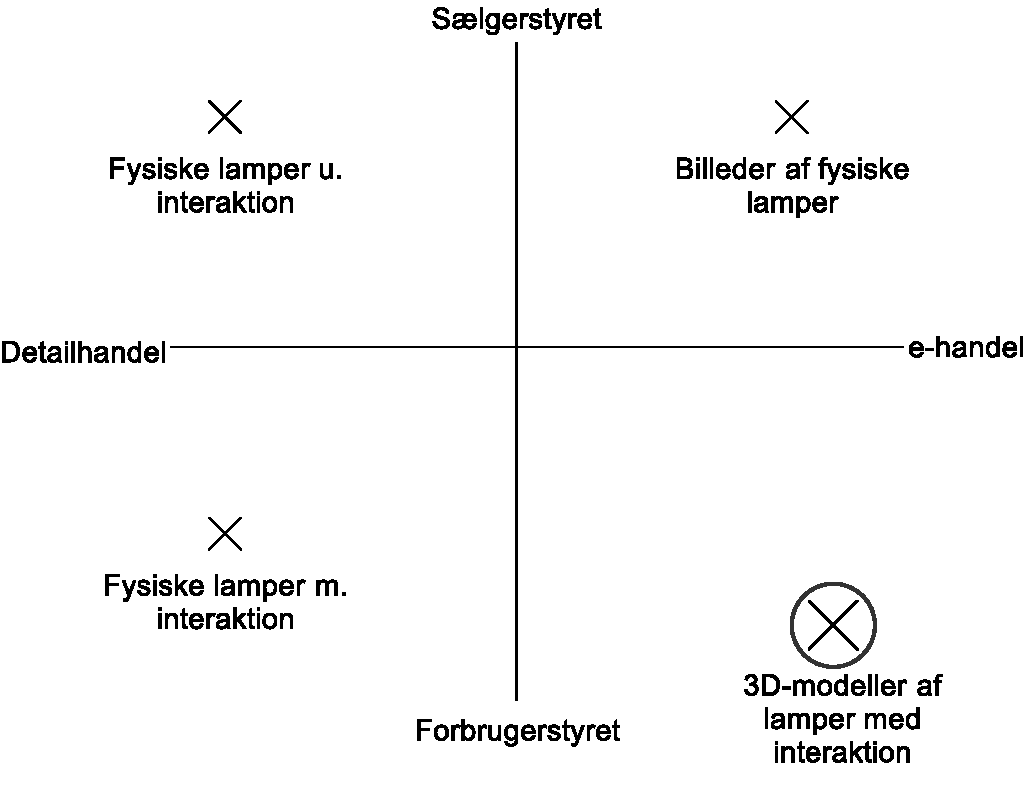
\includegraphics[width=10cm]{p1_skitser}
  \caption{Illustrerer lønningsfeltet til initierende problem, hvor det afgrænsede løsningsfelt er markeret med en cirkel.}
  \label{fig:p1_skitser}
\end{figure}

Herunder er de fire løsningsmuligheder, vist på figur \ref{fig:p1_skitser}, beskrevet:
\begin{enumerate}
  \item fysiske lamper uden interaktion, som er de lamper lampebutikker udstiller i fysiske butikker, men som forbrugeren ikke har mulighed for interaktion med, det vil sige at dette ofte er lamper som er slukket.

  \item fysiske lamper med interaktion, som er de lamper lampebutikker udstiller i fysiske butikker og som brugeren bla. kan slukke og tænde for, altså have interaktion med.

  \item billeder af fysiske lamper på e-butikker. Her har kunden mulighed for at se et billede af lampen, men kun fra de vinkler og i den kontekst som lampebutikken har valgt.

  \item 3D-modeller af fysiske lamper m. interaktion på e-bukker. Her har kunden mulighed for at se et 3D billede af lampen samt rotere lampen, og herved se hvordan lampens belysning er fra de ønskede vinkler, og ikke kun i den kontekst som lampebutikken vælger det. 
\end{enumerate}

Figuren viser nu at det er løsningsmulighed 4, som der afgrænset til i løbet af problemanalysen, og vi dermed har fravalgt løsningsmulighed 1-3 på baggrund af problemanalysen. Dette gør at der nu kan opstilles en endelig problemformulering, som ligger op til en løsningsmulighed 4.